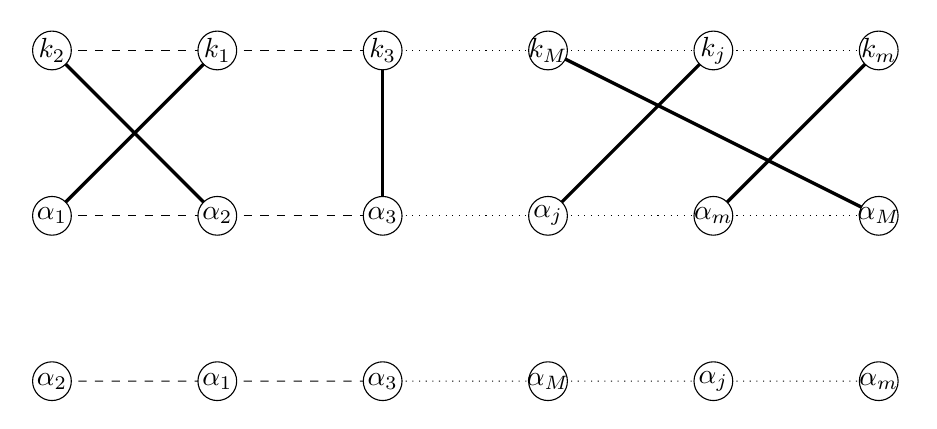
\begin{tikzpicture}[scale=0.7]


\node (alfaPR1) at (-10,-9) {};
\node (alfaPRM) at (5,-9) {};
\node (alfaPR2)at (-7,-9) {};
\node (alfaPR3) at (-4,-9) {};
\node (alfaPR4)at (-1,-9) {};
\node (alfaPR5)at (2,-9) {};

\node (alfaP1) at (-10,-6) {};
\node (alfaPM) at (5,-6) {};
\node (alfaP2)at (-7,-6) {};
\node (alfaP3) at (-4,-6) {};
\node (alfaP4)at (-1,-6) {};
\node (alfaP5)at (2,-6) {};

\node (kp1) at (-10,-3) {};
\node (kpM) at (5,-3) {};
\node (kp2)at (-7,-3) {};
\node (kp3) at (-4,-3) {};
\node (kp4)at (-1,-3) {};
\node (kp5)at (2,-3) {};



\draw[very thick]  (alfaP2) --(kp1);
\draw[very thick]  (alfaP1) --(kp2);
\draw[very thick]  (alfaP3) --(kp3);
\draw[very thick]  (alfaPM) --(kp4);
\draw[very thick]  (alfaP4) --(kp5);
\draw[very thick]  (alfaP5) --(kpM);



\draw [dashed] (kp1) --(kp2);
\draw [dashed] (kp2) --(kp3);
\draw[dotted]  (kp3) --(kp4);
\draw[dotted]  (kp4) --(kp5);
\draw  [dotted](kp5) --(kpM);

\draw  [fill= white](kp1)circle (10pt);
\draw  [fill= white](kpM)circle (10pt);
\draw  [fill= white](kp2)circle (10pt);
\draw  [fill= white](kp3)circle (10pt);
\draw  [fill= white](kp4)circle (10pt);
\draw  [fill= white](kp5)circle (10pt);

\node[] at (kp1)  {$k_2$};
\node[] at (kpM)  {$k_m$};
\node[] at (kp2)  {$k_1$};
\node[] at (kp3)  {$k_3$};
\node[] at (kp4)  {$k_M$};
\node[] at (kp5)  {$k_j$};

\draw[dashed]  (alfaP1) --(alfaP2);
\draw[dashed]  (alfaP2) --(alfaP3);
\draw[dotted]  (alfaP3) --(alfaP4);
\draw[dotted]  (alfaP4) --(alfaP5);
\draw [dotted](alfaP5) --(alfaPM);

\draw[dashed]  (alfaPR1) --(alfaPR2);
\draw[dashed]  (alfaPR2) --(alfaPR3);
\draw[dotted]  (alfaPR3) --(alfaPR4);
\draw[dotted]  (alfaPR4) --(alfaPR5);
\draw [dotted](alfaPR5) --(alfaPRM);

\draw  [fill= white](alfaP1)circle (10pt);
\draw  [fill= white](alfaPM)circle (10pt);
\draw  [fill= white](alfaP2)circle (10pt);
\draw  [fill= white](alfaP3)circle (10pt);
\draw  [fill= white](alfaP4)circle (10pt);
\draw  [fill= white](alfaP5)circle (10pt);

\draw  [fill= white](alfaPR1)circle (10pt);
\draw  [fill= white](alfaPRM)circle (10pt);
\draw  [fill= white](alfaPR2)circle (10pt);
\draw  [fill= white](alfaPR3)circle (10pt);
\draw  [fill= white](alfaPR4)circle (10pt);
\draw  [fill= white](alfaPR5)circle (10pt);

\node[] at (alfaP1)  {$\alpha_1$};
\node[] at (alfaPM)  {$\alpha_M$};
\node[] at (alfaP2)  {$\alpha_2$};
\node[] at (alfaP3)  {$\alpha_3$};
\node[] at (alfaP4)  {$\alpha_j$};
\node[] at (alfaP5)  {$\alpha_m$};

\node[] at (alfaPR1)  {$\alpha_2$};
\node[] at (alfaPRM)  {$\alpha_m$};
\node[] at (alfaPR2)  {$\alpha_1$};
\node[] at (alfaPR3)  {$\alpha_3$};
\node[] at (alfaPR4)  {$\alpha_M$};
\node[] at (alfaPR5)  {$\alpha_j$};
\end{tikzpicture}